\documentclass[12pt,
border=1pt]{standalone}
\usepackage{pgfplots}
\usepackage{amsmath}
\usepackage{amssymb}

\pgfplotsset{compat=newest,
	width=6cm, height=5cm,
	xtick pos=left, ytick pos=left,
	%            scaled x ticks=real:1e-6,
}
% Kernel 2 FP64
\begin{document}
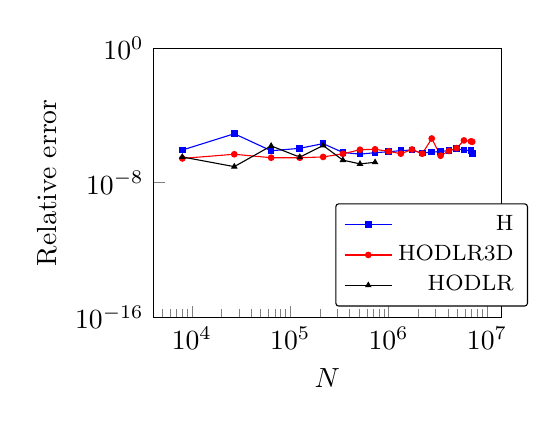
\begin{tikzpicture}[every mark/.append style={mark size=1pt}]
	\begin{axis}[xlabel={$N$},
	ylabel={Relative error},
%		legend pos=south east,
		legend style={
                at={(0.8,0.04)},
               anchor=south,
               legend columns=1,
               cells={anchor=east},
              font=\footnotesize,
               rounded corners=1pt,
               },
		xmode = log,
	    ymode = log,
	   % xmin = 1e3,
	   % xmax = 1e6,
	    ymin = 1e-16,
	    ymax = 1e-0,
	   % xtick={1e-10, 1e-8, 1e-6,  1e-4,  1e-2},
	   % ytick={1e-8, 1e-6,  1e-4,  1e-2, 1e-0}
		]
% 		\addplot[
% 		color=red,
% 		mark=o,
% 		] coordinates {

% (13824,2.031870e-07)
% (110592,1.264230e-07)
% (884736,1.085520e-07)
% (7077888,1.004550e-07)
% 		};
		\addplot[
		color=blue,
		mark=square*,
		] coordinates {
(8000,8.781170e-07)
(27000,8.181320e-06)
(64000,7.946040e-07)
(125000,1.113950e-06)
(216000,2.113240e-06)
(343000,6.333840e-07)
(512000,5.006640e-07)
(729000,6.115090e-07)
(1000000,6.981040e-07)
(1331000,8.089660e-07)
(1728000,8.762710e-07)
(2197000,5.748790e-07)
(2744000,6.699870e-07)
(3375000,7.094760e-07)
(4096000,8.286130e-07)
(4913000,1.061750e-06)
(5832000,8.717860e-07)
(6859000,7.981120e-07)
(7077888,5.521490e-07)
		};
		\addplot[
		color=red,
		mark=*,
		] coordinates {
(8000,2.791760e-07)
(27000,4.940570e-07)
(64000,3.074780e-07)
(125000,3.070430e-07)
(216000,3.419200e-07)
(343000,5.240070e-07)
(512000,9.188420e-07)
(729000,9.728950e-07)
(1000000,7.314820e-07)
(1331000,5.318200e-07)
(1728000,9.487780e-07)
(2197000,5.292880e-07)
(2744000,4.261560e-06)
(3375000,4.043310e-07)
(4096000,7.805670e-07)
(4913000,1.150470e-06)
(5832000,3.285690e-06)
(6859000,2.886940e-06)
(7077888,2.725030e-06)
		};
		
		\addplot[
		color=black,
		mark=triangle*,
		] coordinates {
(8000,3.412190e-07)
(27000,9.071260e-08)
(64000,1.543320e-06)
(125000,3.322150e-07)
(216000,1.630430e-06)
(343000,2.205170e-07)
(512000,1.318990e-07)
(729000,1.639850e-07)
		};		
		\legend{H, HODLR3D, HODLR}
	\end{axis}
\end{tikzpicture}
\end{document}